\chapter{DCF controller}
\section{Inleiding}
De basis van onze wekker wordt gelegd door een klok. Uit dit onderdeel, genaamd DCF-controller,  komt verschillende data, als de tijd, de datum en het weeknummer. Van de tijd uitgang wordt verwacht dat deze gesynchroniseerd met het DCF-signaal is, maar mocht het signaal uitvallen moet de tijd door blijven tellen.
Een van de eigenschappen van deze klok zal zijn dat hij gesynchroniseerd wordt met een zogenaamd DCF-signaal. Dit is een signaal dat in duitsland verzonden wordt en allerlei informatie bevat, als de actuele tijd en de datum. Wij zullen meerdere van deze elementen gebruiken in onze wekker.  Al deze data wordt verzonden door middel van een pulssignaal. Vanuit Duitland wordt elke seconde een puls van 100 of 200 ms verstuurd, zodat respectievelijk een 0-bit en een 1-bit doorgegeven wordt. Dit resulteert in een totaal van 59 bits, gevolgt door een seconde ‘rust’, dat elke minuut opnieuw verzonden wordt. In figuur \ref{fig:Blokdiagram} is te zien welke secondes welke informatie bevatten. In de afbeelding wordt een aantal keer P\# genoemd. Dit zijn paritychecks om het ingekomen signaal te controleren. Als de voorgaande bits een even aantal logische enen bevat, zal de parity bit een logische 0 geven. \emph{\color{red} \#\# Controleren \#\#}

\begin{figure}[h!]
\center
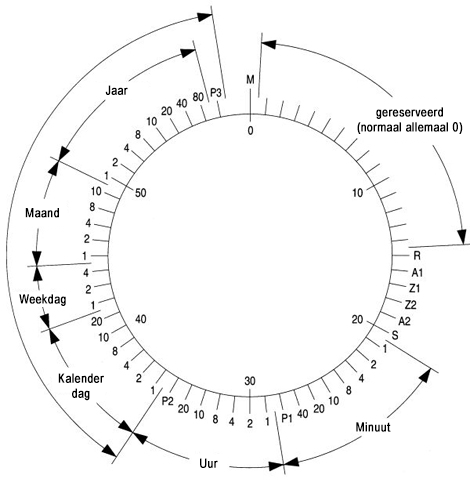
\includegraphics[scale=2]{Figuren/DCF77/dcf77coding.png}
\caption{Codering van het dcf-signaal}
\label{fig:dcfsignaal}
\end{figure}

\section{Specificaties}
In deze sectie zullen we de in- en uitgangen van de DCF-controller in een overzicht weergeven. Doordat het totale systeem met dit onderdeel start, bevat dit blok enkel standaard ingangen en een ingang van buitenaf. De uitgangen uren en minuten worden doorgestuurd naar de main-controller. De clk van 1 Hz zal in verschillende onderdelen worden gebruikt. De debug\_led zal rechtstreeks op het LCD worden weergegeven. 
\subsection{Ingangen}
Dit onderdeel maakt gebruik van de volgende ingangen: 

\begin{itemize}[nolistsep]
\item Reset, standaard input.
\item Klok, standaard input.
\item DCF, signaal van 'logische' pulsen.
\end{itemize}
\noindent

\subsection{Uitgangen}
Dit onderdeel heeft de volgende uitgangen:
\begin{itemize}[nolistsep]
\item Uren, een BCD vector van 6 bits.
\item minuten, een BCD vector van 7 bits.
\item clk, een clk die elke seconde een puls geeft.
\item debug\_led, een signaal dat een logische 1 doorgeeft zodra er een dcf signaal wordt ontvangen.
\end{itemize}


\section{Gedrag}
 De uren en minuten van dit signaal zullen gebruikt worden om de tijd van een interne klok bij te werken. Daarnaast zal de dag van de week, de dag van de maand, de maand en het jaar doorgegeven naar de andere onderdelen van de wekker doorgegeven.
